\cleardoublepage
\chapter{文献综述}

\section{背景介绍}
\par 在全世界范围内,宫颈癌在常见的癌症中位列第四。其也在女想常见的癌症死因中位列第四。\cite{wild2014world}根据WHO组织2014年发布的癌症报告,2012年估计有52.8万例宫颈癌病例,并造成了大约26.6万人死亡。\cite{wild2014world}。宫颈癌在我国也是发病率和病死率很高的女性生殖道恶性肿瘤,数据显示我国女性宫颈癌的原始发病率约为$16.56$($\times 10^{-5}$),位列于乳腺癌($45.29$),肺癌($39.78$),结肠癌($24.25$),甲状腺癌($22.56$)与胃癌($18.15$),高居第五位。\cite{2015癌症报告}
\par 而全世界大约七成的宫颈癌发生在发展中国家\cite{wild2014world},在发达国家中,因为宫颈抹片筛查以及其他检测方法的普及,宫颈癌的发病率和致死率大大降低。\cite{canavan2000cervical}由此说明,定期进行科学的宫颈癌筛查是十分必要的。
\par 宫颈癌筛查主要由“细胞学-阴道镜-组织学”三阶梯诊断程序组成,其中,细胞学筛查的主要手段就是TCT检查,即采用液基薄层细胞检测系统检测宫颈细胞并进行细胞学分类诊断。TCT检查需要医生使用专门的宫颈刷来采集子宫颈的脱落细胞样本,再将细胞样本漂洗后转移到保存液瓶中,然后放入全自动细胞检测仪中将细胞混匀、过滤、转移,并最后将细胞帖附到玻片上。之后需要将玻片进行染色固定才能在显微镜下进行观察诊断。
\par 诊断通常需要医生通过显微镜在整个玻片上寻找疑似病变或病变细胞,最后根据全片病变细胞的状况给出诊断。但是,在临床实践的过程中可能会遇到许多问题。

\begin{enumerate}
    \item TCT检查图片巨大
          \par 如\ref{全片}所示,整个TCT样本的片子十分巨大,玻片上细胞数目也非常多,检阅全片需要非常大的工作量。

          \begin{figure}[h]
              \centering
              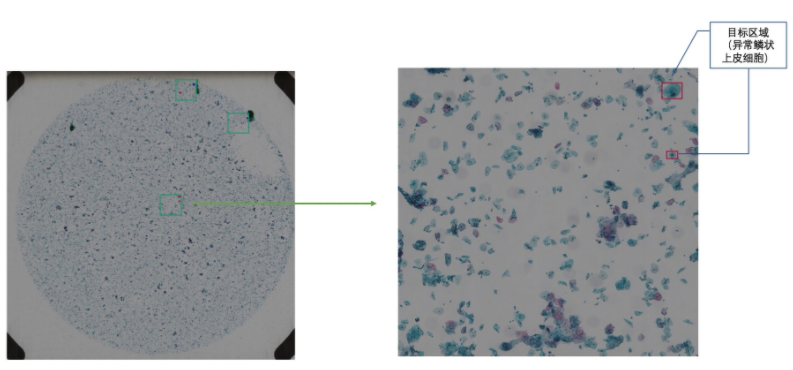
\includegraphics[width=0.5\paperwidth]{TCT/whole_pic.png}
              \caption{全片与部分视野的大小对比。左图为全片,右图为一个视野,在视野中可以看到正常细胞与病变细胞}
              \label{全片}
          \end{figure}
    \item 遗漏病变细胞
          \par 因为上述的涂片巨大的问题,在临床实践中很可能会遗漏病变细胞,从而影响诊断结果的准确性。例如,如果医生在阅片时遗漏了某个病变等级较高的细胞聚集的区域,那么诊断结果可能会更倾向于较低的病变等级,这显然不利于医生做出准确的诊断结果也不利于医生和患者获悉正确的病情。而且,这一过程使得诊断结果具有了一定的随机性,时期不能准确描述患者的病情。
    \item 类别判定的主观性
          \par 此外,全人工的阅片或检阅部分视野可能会导致诊断结果的主观性过强,某些类别的判定可能没有十分明确的标准导致医生在诊断时诊断结果取决于医生的主观偏好。以\ref{HSIL-SQCA}为例,可以看到右图中部分被标注为HSIL的病变区域有着与SQCA区域几乎相同的形态特征而与左图中的HSIL类别的形态差异较大。这是因为在临床实践中,SQCA类别的检出更依赖于组织病理切片而不是TCT检查,所以医生在判定这两种类别时主观性就比较强,医生对于某些勉强达到SQCA标准的病变细胞,就更愿意标注为HSIL而不是SQCA。

          \begin{figure}[h]
              \centering
              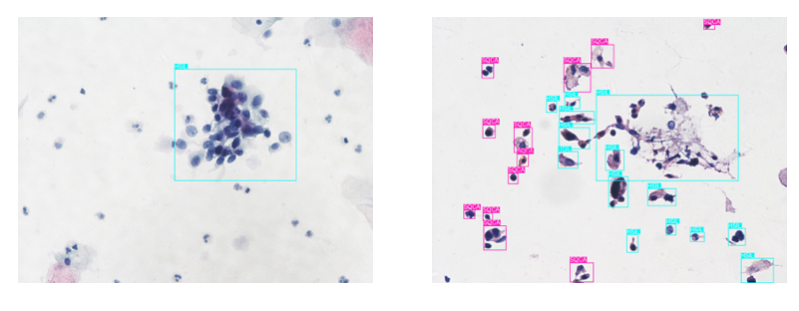
\includegraphics[width=0.5\paperwidth]{TCT/HSIL-SQCA.png}
              \caption{HSIL与SQCA两个类别的特征,左图为HSIL,右图为SQCA。全片与部分视野的大小对比。}
              \label{HSIL-SQCA}
          \end{figure}
\end{enumerate}
\par 由此,宫颈TCT的筛查亟需计算机的辅助诊断方法以实现快速、准确的宫颈癌筛查,以减少医生的工作量,避免诊断过程中因为人为原因造成遗漏等问题,并进一步提高诊断结果的准确性。

\section{国内外研究现状}
\par 目前国内外通过计算机辅助医生进行宫颈TCT检测的方法主要分为病变细胞分类、病变细胞检测、病变部位分割三个部分。
\par 病变细胞分类主要是指仅给出输入视野中细胞的综合病变等级,一般会根据病变细胞的状况评定为在视野中出现的最高病变等级或者次高级。以\ref{样例图片}为例,在病变细胞分类的任务中,计算机仅需要指出图片中最高级的病变细胞种类——HSIL即可。
\par 病变细胞检测则是要求以矩形框的方式标注出视野内的病变细胞并给出病变等级,相较病变细胞分类任务而言,评定整个视野的综合病变等级的任务由医生完成。在病变细胞检测的任务中,计算机应当标注出所有病变细胞的位置并给每个病变细胞评定病变等级,结果应如\ref{样例图片}中间部分图片
\par 病变细胞分割则是在病变细胞检测的基础上,要求以像素级的精度标注出病变细胞的范围。病变细胞分割的任务中,计算机标注病变细胞位置的结果应当更为精确,例如图\ref{样例图片}右面部分。

\begin{figure}[h]
    \centering
    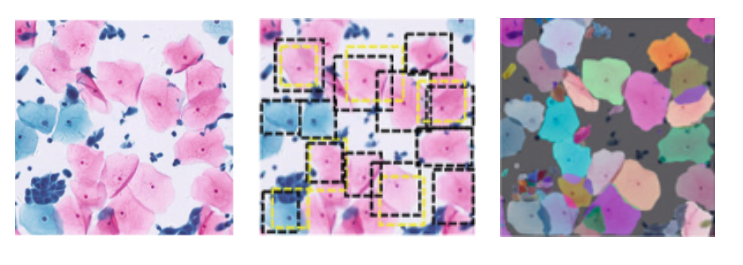
\includegraphics[width=0.5\paperwidth]{TCT/example_res.png}
    \caption{样例图片与其检测、分割任务的结果,左图为样例图片,中间是样例图片的检测结果,右图为样例图片的分割结果}
    \label{样例图片}
\end{figure}

\subsection{研究方向及进展}

\subsubsection{病变细胞分类与分割}
\par 在临床实践中,医生主要依据细胞核与细胞质的比例,细胞核的大小,细胞核的形状以及核膜的异常变化来判定病变的宫颈细胞,以及区分它们的种类。因此,有许多研究\cite{zhang2014segmentation}\cite{zhang2017graph}\cite{lee2016segmentation}通过分割细胞或细胞的某些部分(细胞核、细胞质),并依据临床上的判定规则完成病变细胞的分类任务。但是由于不同种类细胞的形态差异较大、细胞之间的重叠问题可能比较严重以及细胞质边界可能不够清晰等问题,细胞以及细胞成分的分割依然是一个尚未被很好解决的问题。因此,这类方法往往不能让人满意。
\par 而在另一方面,也有许多研究\cite{marinakis2009pap}\cite{phoulady2016automatic}通过手工设计大量的特征试图捕捉细胞核和细胞质的形态特征,再将这些特征经过特征选择或者降维处理之后输入到各种分类器中(如,随机森林、SVM、神经网络等)来完成分类任务。但是,上述的手工设计的特征往往依赖于细胞或细胞组成成分的分割结果,而且这些手工设计的特征完全来自于当前医学对于宫颈细胞学的认知,因此,此类方法的发展会受到医学发展的限制。
\subsubsection{病变细胞检测}
\par 近期,病变细胞检测方向的研究主要是基于卷积神经网络进行的。这种基于卷积神经网络的方法一开始被应用在自然图像上,Overleaf\cite{sermanet2013overfeat}最早将卷积神经网络应用到目标检测任务上,它与当时基于手工设计特征的方法相比,有50\%以上的mAP增幅。随后,又有许多基于卷积神经网络的方法出现。例如,Fast R-CNN\cite{girshick2015fast}、Faster R-CNN\cite{ren2015faster}、Mask R-CNN\cite{he2017mask}系列,以及yolo系列\cite{redmon2016you}\cite{redmon2017yolo9000}等。他们大致可以分为两类:基于图像提案的方法\cite{ren2015faster}\cite{girshick2015fast},以及无提案的方法\cite{redmon2016you}\cite{redmon2017yolo9000}。一般来说,基于图像提案的方法会首先提起一些图像提案,再经过一系列的过程优化这些提案,这类方法在准确性方法往往会更具优势。而无提案的方法往往直接预测边界框与目标类别,它们往往具有更快的速度,但准确性上会略逊一筹。在处理TCT图像时我们往往更关注检测结果的准确性和召回率,而忽视其检测速度差异,因此,这方面的研究往往基于图像提案来完成。
\par 除此之外,由于卷积神经网络的学习往往需要大量的标注数据,而TCT图像的标注结果是由专业的医师来完成的,那么获取大量的数据就会带来高额的成本,因此也有许多研究\cite{ou2020semi}通过一些半监督的方法来利用大量无标注信息的图像促进网络的学习。
\par 目前病变细胞检测方面相关的论文、其所使用的方法、数据集以及最终效果(部分)如\ref{检测论文}:
\begin{table}[htbp]
    \center
    \tiny
    \caption{病变细胞检测论文汇总}
    \begin{tabular}{p{120pt}p{100pt}p{85pt}p{35pt}}
        \hline
        论文                                                             & 模型                         & 数据                       & 效果(mAP) \\
        \hline
        MACD R-CNN\cite{ma2020macd}                                      & 基于mask R-CNN 的 MACD R-CNN & Herlev 数据集              &             \\
        Automation-Assisted Reading Method\cite{xiang2020novel}          & YOLO V3 和额外的分类器       & 私有数据12909 例,10个类别 & 0.634       \\
        Detection in the Limited Data Scenario\cite{liang2018comparison} & Faster R-CNN + FPN           & 私有数据7086例,11个类别   & 0.263       \\
        Detection and Classification of Cells\cite{li2019detection}      & Faster R-CNN                 & 680例,6个类别             &             \\
        Multitask Learning for Recognition\cite{liu2018multitask}        & VGG16                        & 73 例                      &             \\
        DCCL\cite{zhang2019dccl}                                         & Faster R-CNN,RetinaNet      & DCCL公开数据               &             \\
        \hline
    \end{tabular}
    \label{检测论文}
\end{table}

\subsection{存在问题}
\subsubsection{染色问题}
\par TCT检查的视野中细胞各个部分的颜色并不是细胞本身的颜色,而是染色剂染色之后的颜色。因此,即使是同样的细胞部位、同样的病变程度,也可能因为染色剂的不同而呈现出不同的颜色状态。不仅如此,输入到计算机中的视野图片并不一定是TCT检查刚刚做完时的视野图片,而染色剂会随着时间慢慢褪色。不同染色剂品牌,不同颜色的染色剂都会有不同的褪色速率,因此,即使是同一张视野图片也可能因为输入计算机系统的时间不同而表现出不同的色彩状态。
\subsubsection{标注框问题}
\par 医生在标注病变细胞框的时候,如果病变细胞是单个存在的、周围没有其他细胞的状态,那么医生会给该细胞单独标注一个框。但是,如果病变细胞聚集在一起形成了一个很大的细胞团,那么病变细胞之间的界限会变得十分糢糊,只能选择标注一个很大的框将整个细胞团框住。这就导致了同一种类标签的标注框有着两种不同的含义——既可以是单个的病变细胞,也可以是一整个病变细胞团,而二者在形态上有着巨大的差异。
\par 例如,由于不论是病变细胞还是正常细胞细胞核往往在形态上处在整个细胞中心的位置,那么单个细胞对应的框的中心一般来说就是这个细胞的细胞核,因此从该处往往可以获得细胞核的形态特征。换句话说,如果网络发现了细胞核的形态特征,就可以将该点作为检测框的中心的进行预测。但是,如果框中的是一个大的细胞团那么其中心就不再是明显的细胞核的特征了。而细胞核的形态特征又是判断病变与否已经病变种类的相当关键的特征,这就导致网络的学习过程中可能遇到难以学习的特征形态。与此类似的,单个细胞框的周围会是细胞质边界的特征,这也是判断病变细胞的一个重要特征,但是细胞团的边缘是多个细胞聚集在一起时组成的形状,因为细胞是经过混匀的,这一形态信息完全由混匀过程决定可以认为是随机的,这对判断细胞的病变程度毫无意义。
\par 此外,单个细胞与细胞团的界限并没有那么明显。例如,医生在标注框的时候,会遇到两三个细胞挨在一起的情况,这种情况下可以说为每个细胞单独标注框和将这两三个细胞视作一个细胞团只标注一个框都是合理的。但这就给网络的学习带来了很大的难度——网络不仅要学会如何判断病变细胞,还需要学会制作训练用数据集的医生对于上述情况的偏好情况。而事实上,由于数据的标注由不止一位医生完成,往往每位医生对都上述情况会有不同的偏好,因此,网络可能根本无法学习到这一规律。这一问题严重地阻碍了网络的学习过程,然而,在实践中,我们往往并不关注病变细胞是有单独的框还是由一个框标注出来的,我们更关心病变细胞的召回率和病变等级判定的准确率。
\subsubsection{放大倍率不统一}
\par TCT检查的图片都是经过显微镜放大的,所以图片中细胞的绝对大小并没有实际的意义,甚至这一大小的变换还会为网络的学习带来阻碍。例如,涂片中可能出现一种叫做炎细胞的正常细胞,它相比入一般细胞会小得多,医生在做诊断时可以自然地忽略它,但是它的形态特征在放大之后与最高等级的病变细胞——鳞癌细胞的形态特征十分相近。他们的区别只是炎细胞相较与正常细胞非常小,而鳞癌细胞具有正常细胞的大小尺度。现有的深度学习方法主要通过FPN来生成各种尺度的图像金字塔来处理这种尺度变换的问题,但是,这种方法更适合用来检测尺度大小不确定的目标,对于形态特征相近只有尺度不同的目标,这种方式反而会影响网络的训练。
\subsubsection{样本数量过少}
\par 有许多病变细胞检测方向的研究都是基于卷积神经网络的,这就需要大量的训练数据。而TCT检查的标注数据需要由专业的医师来完成,这就导致可以获取到的标注数据很少,请医生完成标注又可能遇到成本过高的问题。因此,如何更好得利用无标注的数据促进模型的学习是亟待解决的问题。

\section{研究展望}
\par 我们基于上述问题,希望通过不同的方法尝试解决或者缓解上述问题对网络学习的影响。

\subsection{标注框问题}
\par 我们希望通过对数据标注的重新整理和重新标注区分出单个细胞的框和细胞团对应的框,并分别使用不同的网络结构来预测他们。

\subsection{放大倍率不统一}
\par 我们在与医生沟通之后,了解到医生在标注图片、诊断病例的过程中往往会依靠视野中的正常细胞大小来作为基准,以此来判断病变细胞的大小。其中,正常细胞的细胞核大小和细胞质大小是十分重要的判断依据,医生主要通过对比病变细胞与正常细胞的细胞核大小、细胞质大小来判定病变程度。因此,我们希望模仿医生判断的过程,让网络可以先识别一些正常细胞,然后依据正常细胞的形态、尺寸信息来帮助病变细胞的识别与类别判定。

\subsection{样本数量过少}
\par 我们希望通过引入半监督学习中知识蒸馏等方法,让模型更好地利用无标注的数据完成训练。

\newpage
\begingroup
\linespread{1}
\printbibliography[title={参考文献}]
\endgroup
